\chapter{Criptografía Asimétrica y Curvas Elípticas. RSA y Diffie-Hellman}
En esta capítulo voy a explicar de los criptosistemas asimétricos usados en las aplicaciones de mensajería hoy en día. Primero describiré el funcionamiento del cifrado RSA y la firma digital usando este. Después explicaré el problema del Logaritmo Discreto y el intercambio de claves \emph{Diffie-Helmman}. Y por último concluiré haciendo una introducción a la teoría de Curvas Elípticas, el problema del Logaritmo Discreto en estas y por último el intercambio de claves \emph{Diffie-Hellman} usando Curvas Elípticas.\\

\section{Criptosistema de Rivest-Shamir-Adleman, RSA}
RSA es llamado así en honor a sus creadores Ron Rivest, Adi Shamir y Loenard Adleman. Fue desarrollado en 1977. Cabe a destacar que en 1973 se desarrolló en secreto un criptosistema similar por Clifford Cocks para la \emph{Government Communications Headquarters}, que es la agencia de inteligencia de señales británica, y fue desclasificado en 1997\cite{cliffordCocks}.\\
Este criptosistema está basado en el \emph{Teorema de Euler} y en particular en la \emph{Proposición 2.2}.\\


\begin{teorema}
	(Teorema de Euler) Sean a,n $\in \mathbb{Z}$ primos relativos entre sí, entonces $a^{\phi(n)}\equiv 1 \mod n$.
\end{teorema}\vspace*{-7mm}
\begin{proof}
		Sea $n\in \mathbb{Z^+}$ que verifica que $\operatorname{mcd}(a,n)=1$ y definimos $S$ como el conjunto de las unidades modulo $n$, $S=\{u_1,u_2,\dots,u_{\phi(n)}\}$ donde $1\leq u_i\leq n-1$, $\operatorname{mcd}(u_i,n)=1$ y $u_i\neq u_j$ $\forall i,j \in \{1,\dots,\phi(n)\}$ con $ i\neq j$.\\
	Multiplicando  los elementos de $S$ por $a$ obtenemos 
	$$
		aS=\{au_1,au_2,\dots,au_{\phi(n)}\}
	$$
	Como $\operatorname{mcd}(a,n)=1$ entonces $a\mod n$ es una unidad y por tanto $aS$ será el conjunto de las unidades módulo $n$. Y dado que los elementos de $S$ y los de $aS$ coinciden módulo $n$, el producto de estos será el mismo módulo $n$ por lo que obtenemos 
	$$
		u_1u_2\dots u_{\phi(n)} \equiv (au_1)(au_2)\dots (au_{\phi(n)})\mod n.
	$$
	Sacando como factor común $a$ tenemos 
	$$
		u_1u_2\dots u_{\phi(n)} \equiv a^{\phi(n)}u_1u_2\dots u_{\phi(n)}\mod n. 
	$$
\end{proof}\\

\begin{teorema}
		(Teorema pequeño de Fermat) Sea $a \in \mathbb{Z}$ y $p$ un número primo tal que $\operatorname{mcd}(a,p)=1$. Entonces
	$$
		a^{p-1} \equiv 1 \mod p.
	$$
\end{teorema}\vspace*{-7mm}
\begin{proof}
		Sea $a \in \mathbb{Z}$. Tomamos los $p-1$ primeros múltiplos positivos de $a$ que serán de la forma $a, 2a,\dots,(p-1)a$. El resto resultante de dividir los $p-1$ múltiplos positivos de $a$ por $p$ corresponden a 1,2,3,$\dots,p-1$.\\
	Multiplicando ahora todas las congruencias obtenemos 
	$$
		a^{p-1}·(p-1)! \equiv (p-1)! \mod p.
	$$
	Como tenemos que $p\nmid (p-1)!$ se cumple que $\operatorname{mcd}(p,p-1)=1$ y por tanto cancelando en la expresión anterior obtenemos
	$$
		a^{p-1} \equiv 1 \mod p. 
	$$
\end{proof}

Cabe a mencionar que el Teorema de Fermat es un caso particular del Teorema de Euler.\\
\begin{definicion}
Se conoce a la función $\phi(n)$ como la función de Euler. Esta es definida como $\phi(n)=|\mathbb{Z}^*_n|$ y se puede calcular como $$\phi(n)=n\prod_{p_i|n}\left(1-\frac{1}{p_i}\right).$$
\end{definicion}

\begin{teorema}
		(Teorema Chino del Resto) Sean $a_1, a_2\in \mathbb{Z}$ y $p,q \in \mathbb{N}$ tales que $\operatorname{mcd}(p,q) = 1$. Entonces el sistema
		$$
			x\equiv a_1 \mod p,
		$$\vspace*{-11mm}

		$$
			x\equiv a_2 \mod q,
		$$
	tiene solución única módulo $n=pq$. Además, la solución está dada por
	$$
		x\equiv a_1\cdot q\cdot d_1 +a_2\cdot p\cdot d_2 \mod n,
	$$
	donde se cumple
	$$
		q\cdot d_1 \equiv 1 \mod p,
	$$
	$$
		p\cdot d_2 \equiv 1 \mod q.
	$$
\end{teorema}
\begin{proof}
		Veamos la existencia de la solución. Sea $N=p\cdot q$. Como por hipótesis tenemos que $\operatorname{mcm}(p,q)=1$, por Bézout existen enteros $d_i$, $s_i$ con $i=1,2$ tales que $d_1p+s_1q=1$ y $d_2q+s_2p=1$. Tomando módulo $p$ y $q$ tenemos que 
	$$
		d_1\cdot p \equiv 1 \mod q,
	$$
	$$
		d_2\cdot q \equiv 1 \mod p.
	$$
	Definiendo 
	$$
		x :=  a_1\cdot q\cdot d_1 +a_2\cdot p\cdot d_2,
	$$
	se consigue que $x$ sea la solución del sistema. Además, trabajando módulo $p$ y $q$ obtenemos que $x\equiv a_1 \mod p$ y $x\equiv a_2 \mod q$.\\
	Una vez vista la existencia de la solución quedaría demostrar la unicidad. Para ello supongamos que existen dos números enteros distintos $x$ e $y$ tales que 
		\begin{equation}
			\begin{split}
				x \equiv a_1 \mod p,\notag\\
				y \equiv a_1 \mod p.\notag
			\end{split}
		\end{equation}
	Y también 
		\begin{equation}
			\begin{split}
				x \equiv a_2 \mod q,\notag\\
				y \equiv a_2 \mod q.\notag
			\end{split}
		\end{equation}
	Esto implica que $x-y\equiv0 \mod p$ y $x-y\equiv0 \mod q$. Como $p$ y $q$ son coprimos, tenemos que $x-y\equiv 0 \mod N$, luego se da que $x\equiv y \mod N$ llegando así a una contradicción. \qedhere
\end{proof}

\begin{proposicion}
	Sea $n = pq$, donde p y q son dos primos distintos. Si $x\equiv 1 \mod \phi(n)$, entonces $a^x\equiv a\mod n$ para todo $ a \n \in \mathbb{Z}$.
\end{proposicion}\vspace*{-5mm}

	\begin{proof}
		Si $a$ es múltiplo de $n$, entonces se cumple que $a^x \equiv 0 \equiv a \mod n$. Si $a$ y $n$ son coprimos, $\operatorname{mcm}(a,n) = 1$. Entonces tendríamos que $a^x \equiv a \mod n$ por el Teorema de Euler.\\
		Nos quedaría ver ocurre en el caso de $a$ sea múltiplo de $p$ o de $q$, pero no de ambos. Por simetría supondremos que a es múltiplo de $p$, pero no de $q$. En este caso tenemos que $a^x \equiv 0 \equiv a \mod p$  y $a^x \equiv a \mod q$ por el Teorema de Fermat. Como $p$ y $q$ son coprimos entre sí, aplicando el Teorema Chino del Resto se deduce que $a^x \equiv a \mod n$.\qedhere
	\end{proof}

Una vez que tenemos herramientas necesarias vamos a describir el funcionamiento de RSA. El contenido de esta sección se basa en \cite{angelRiosMateos}.\\
El usuario elige dos números primos distintos \emph{p} y \emph{q} de buen tamaño ya que mientras más grandes sean más seguro será el cifrado.
Se calcula $n = pq$ y por tanto tenemos que $\phi(n) = (p-1)(q-1)$. A continuación se elige un elemento $c$ coprimo con $\phi(n)$ y se calcula el inverso $d = c^{-1}\mod \phi(n)$. La clave pública será $k=(n,c)$ y la clave privada $k'=(n,d)$.\\
En un principio se consideraba que un tamaño de $n$ de 1024 bits era lo suficientemente grande para que fuera seguro, pero en 2003 Tromer y Shamir mostraron que es posible factorizar números de 1024 bits \cite{1024RSA} por lo que en la actualidad se considera 2048 bits como un tamaño seguro.\\
El conjunto de los mensajes sin cifrar es $\mathcal{M}$, el de los mensajes cifrados será $\mathcal{C}$ y se verifica que $\mathcal{M} = \mathcal{C} = \mathbb{Z}_n$. Las funciones de cifrado y descifrado son respectivamente:
\begin{align*}
	E_{k}:\mathcal{M}\rightarrow\mathcal{C},\\
	a \rightarrow a^c,
\end{align*}
\begin{align*}
	D_{k'}:\mathcal{C}\rightarrow\mathcal{M},\\
	a \rightarrow a^d.
\end{align*}
Como hemos visto anteriormente, el tamaño del mensaje puede llegar a ser un problema ya que aumenta el tiempo de encriptación y desencriptación. Para solucionar esto se puede fragmentar el mensaje y usar métodos de operación en bloques. Lo más habitual es usar funciones resumen, que de hecho, es el método que se sigue en las aplicaciones de mensajería como veremos en el siguiente capítulo.\\
Además RSA puede ser vulnerable en función de los números primos que se elijan y el tamaño de estos. 
Por ejemplo para evitar \textbf{el ataque por módulo común}, es recomendable utilizar distinto módulo $n$ para cada clave. 
Para evitar \textbf{el ataque por exponente pequeño} es recomendable utilizar unos números primos $p$ y $q$ grandes. Ya que si no se usan, se puede utilizar el Teorema Chino del Resto para factorizar $n$ y obtenerlos. 
Para evitar \textbf{el ataque por primos muy próximos} se recomienda usar números primos que estén relativamente alejados entre sí. 

\subsection{Firma digital RSA}
La firma digital con RSA, es una herramienta muy utilizada en las aplicaciones de mensajería para garantizar el no repudio de los mensajes.
Dados dos interlocutores A y B cada uno con sus claves públicas:
\begin{itemize}
	\item para A tenemos $n_A$, $d_A$ y $e_A$,  
	\item para B tenemos $n_B$, $d_B$ y $e_B$.  
\end{itemize}
Para que B sepa que un mensaje \emph{m} ha sido enviado por A se siguen los siguientes pasos.
\begin{enumerate}
	\item A cifra el mensaje \emph{m} usando su clave secreta:
		$$
			S=D_A(m)=m^{d_A} \mod n_A.
		$$
	\item A continuación encripta el mensaje firmado con la clave pública de B:
		$$
			C_B(S)=S^{e_B}\mod n_B.
		$$
		y se lo envía a B.
	\item B recibe $C_B(S)=S^{e_B} \mod n_B$ y lo desencripta: 
		$$
			D_B(S^{e_B})=S \mod n_B.
		$$
	\item Una vez desencriptado la primera parte, B desencripta S con la clave pública de A:
		$$
			C_A(S)=C_A(D_A(m))=(m^{d_A})^{e_A}=m^{d_Ae_B}=m^{1+k\phi(n_A)}\equiv m \mod n_A.
		$$
\end{enumerate}
Una vez hecho esto, B podría afirmar casi con total seguridad que el mensaje ha sido enviado por A garantizando el no repudio del mensaje.\\
Sin embargo este método tiene un inconveniente y es que para documentos muy largos, el proceso para firmar y verificar es muy lento. Para solucionarlo se utiliza una función hash o resumen de manera que en lugar de firmar el mensaje entero, se firma un resumen de este. La firma en este caso quedaría $fir(m)=h(m)^{d_A} \mod n$ y la comprobación sería $h(m)=fir(m)^{d_A} \mod n$ donde $h$ será una función hash o resumen de las que hablaré al final del capítulo.

\section{El Problema del Logaritmo Discreto. Diffie-Hellman}
El intercambio de claves \emph{Diffie-Hellman} es un método basado en el Problema del Logaritmo Discreto muy utilizado en las aplicaciones de mensajería al iniciar una conexión. La información de este apartado sobre el logaritmo discreto ha sido obtenida de \cite{angelRiosMateos} y la de \emph{Diffie-Hellman} ha sido obtenida de \cite{En2011}.\\
El Problema del Logaritmo Discreto es definido de la siguiente forma:
\begin{definicion}
	Sea S un semigrupo finito. El Problema del Logaritmo Discreto en el semigrupo S es el de resolver una ecuación del tipo\\
		$$
			a^x\!=b\;(x\in \mathbb{N}),
		$$
	donde a y b son dos elementos dados de S.
\end{definicion}

La complejidad del Problema del Logaritmo Discreto depende en gran medida del semigrupo $S$ que se elija.
Dado que si se eligiera como $S$ el grupo aditivo $\mathbb{Z}_n$ la solución se obtendría fácilmente resolviendo una ecuación de congruencias del tipo $aX \equiv b \mod n$ que equivaldría a resolver la ecuación diofántica $aX + nY = b$. Pero si ahora $S$ pasara a ser los semigrupos multiplicativos $\mathbb{Z}_n$ o $\mathbb{F}_q$ o sus grupos de unidades, el problema aumentaría su complejidad de manera significativa.\\
Tenemos que $a^x = b$ tiene solución si y solamente si $b$ está en el semigrupo cíclico generado por $a$. Luego si $a$ es un elemento de orden finito de un grupo, se podría suponer en la práctica que $S$ es un grupo cíclico y por ello existiría un isomorfismo con ($\mathbb{Z}_n$, $+$). Luego la dificultad del problema no estaría en la estructura del grupo, sino en reconocer los elementos como potencias de enteros.\\
Se cree que el problema de logaritmo discreto es $\mathbb{NP}$-completo, pero esta conjetura todavía no ha sido demostrada por lo que se considera un problema $\mathbb{NP}$-Intermedio. Estos problemas son llamados así porque no están dentro de los problemas $\mathbb{P}$ ni en los problemas $\mathbb{NP}$-completo \cite{NP-intermedio}.\\
Una vez visto el problema de logaritmo discreto, se explicará el intercambio de claves \emph{Diffie-Hellman}.
\subsection{Intercambio de claves Diffie-Hellman}
Antes de explicar el intercambio de claves \emph{Diffie-Hellman} se introducirá el problema de Diffie-Hellman ya que es la base de este.\\

%\begin{definicion}
	%Dado el conjunto $\mathbb{Z}^*_{p'}$ con p primo, diremos que $\alpha \in \mathbb{Z}^*_p$ es un generador de $\mathbb{Z}^*_{p'}$ si se cumple:\\
	%$$
		%\forall b \in \mathbb{Z}^*_{p'},\: \exists i\: tal \: que \: \alpha^i = b
	%$$
%\end{definicion}

\begin{definicion}
	(El Problema Diffie-Hellman)\\ Dado un número primo p, un número $\alpha$ que sea un \emph{generador} de $\mathbb{Z}^*_{p'}$, $\alpha^a$ y $\alpha^b$, encontrar $\alpha^{ab} \mod p$.  
\end{definicion}

\subsubsection{Intercambio de claves \emph{Diffie-Hellman}}
El intercambio de claves \emph{Diffie-Hellman} es un algoritmo asimétrico basado en el problema de \emph{Diffie-Hellman}, empleado para acordar una clave común en un canal inseguro. Los pasos que se siguen son:\\
Sean $A$ y $B$ dos interlocutores que quieren compartir un valor $K$. Para ello se calcula un número primo $p$ y un generador \alpha de $\mathbb{Z}^*_{p'}$ con $2\leq \alpha \leq p-2$. Esta información es pública y conocida por ambos.
\begin{enumerate}
	\item $A$ escoge un número aleatorio $x$, comprendido entre 1 y $p-2$ y envía a $B$ el valor 
		$$
			\alpha^x \mod p.
		$$
	\item Análogamente $B$ escoge un número aleatorio $y$, comprendido entre 1 y $p-2$ y envía a $A$ el valor 
		$$
			\alpha^y \mod p.
		$$

	\item $B$ recoge $\alpha^x$ y calcula $K=(\alpha^x)^y \mod p$.
	\item $A$ recoge $\alpha^y$ y calcula $K=(\alpha^y)^x \mod p$.
\end{enumerate}
Puesto que $x$ e $y$ son conocidos solamente por $A$ y $B$ respectivamente, tenemos que al final ambos acaban conociendo el valor de $K$.\\

\section{Curvas Elípticas en Criptografía}
A continuación se introducirá la teoría de curvas Elípticas ya que nos permitirá redefinir el intercambio de claves usando estas. Es el método que se usa actualmente en aplicaciones de mensajería que implementan el protocolo \emph{MTProto} y \emph{Signal}.\\
La criptografía en Curvas Elípticas es considerada como uno de los campos con mayor potencial en la criptografía asimétrica.
Esto es debido a sus propiedades que dan lugar a problemas muy complejos análogos a los que presenta la aritmética modular por lo que garantizan más la seguridad. 
Esto permite que sean utilizadas en algunos algoritmos asimétricos como puede ser el intercambio de claves \emph{Diffie-Hellman} que se verá más adelante. 
Aunque su estructura algebraica es más compleja que la de la aritmética modular sin embargo, al implementarlas suelen ser más eficientes y además, con claves más cortas alcanzan 
el mismo nivel de seguridad.\\
El uso de curvas elípticas en criptografía se presentó por primera vez en 1985 por Neal Koblitz y Víctor Miller de manera independiente.\\
La información para esta sección se ha obtenido de \cite{En2011} y de \cite{apuntesCriptografia}.\\

Una curva elíptica $E$ sobre un cuerpo $\mathcal{K}$ es el conjunto de los $(x,y)\in \mathcal{K}^2$ tales que
$$
	y^2+a_1xy+a_3y = x^3+a_2x^2+a_4x+a_6,
$$
junto con un punto $\mathcal{O}$.\\
Un ejemplo de curvas elípticas en $\mathbb{R}$ son:
\begin{figure}[htb]
	\centering
	\subfloat[\centering Curva $y^2=x^3-4x+1$]{{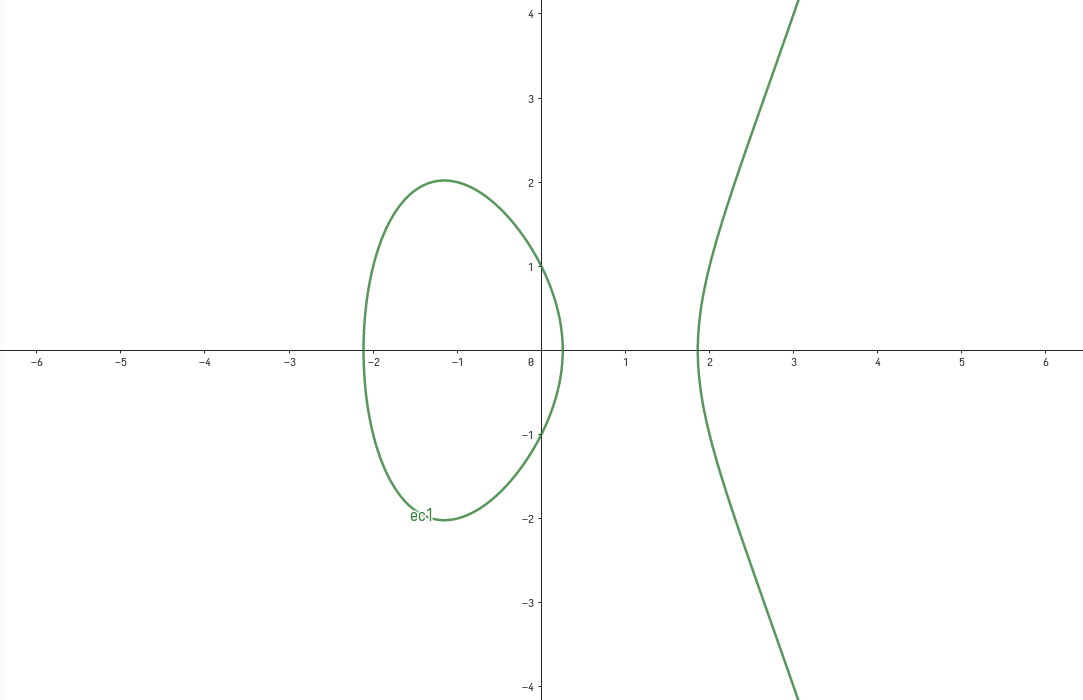
\includegraphics[width=5.9cm]{imagenes/ec1:y^2x^3-4x+1.png}}}
	\qquad
	\subfloat[\centering Curva $y^2=x^3-3x+4$]{{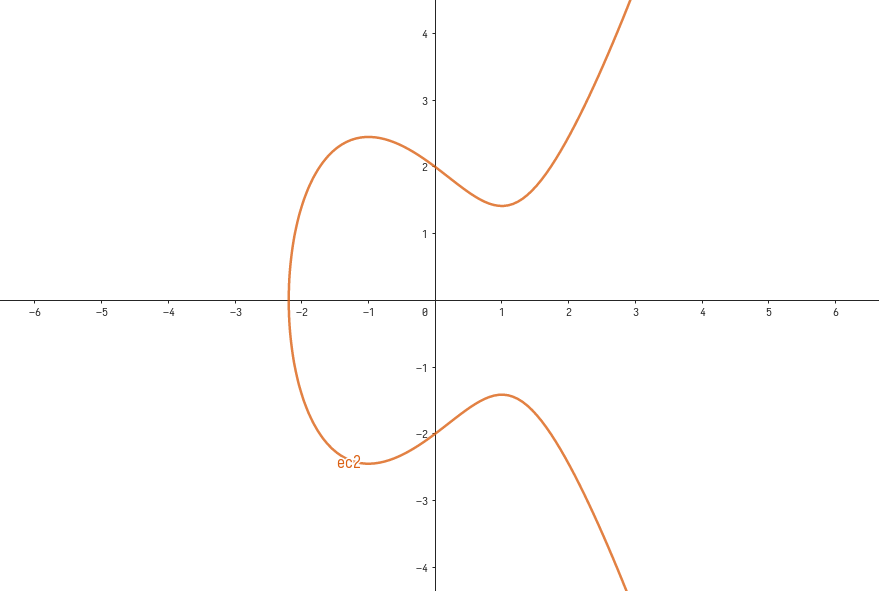
\includegraphics[width=5.9cm]{imagenes/ec2:y^2x^3-3x+4.png}}}
\end{figure}

\begin{proposicion}
		Sea $p=\operatorname{char}(\mathcal{K})$ y sea $E$ una curva elíptica definida sobre $\mathcal{K}$.
		\begin{enumerate}
			\item Si $p$\textgreater$3$, la ecuación $E$ puede simplificarse a
		\begin{align}
			y^2=x^3+ax+b,\label{eq:tipo1}
		\end{align}
		recibiendo el nombre de forma de Weiertrass.
			\item Si $p=3$, la ecuación de $E$ puede simplificarse a 
		\begin{equation}
			y^2=x^3+a^2+bx+c.
		\end{equation}
			\item Si $p=2$ la ecuación de $E$ puede simplificarse a 
				\begin{align}
					y^2+xy=x^3+ax^2+b \: si\: a_1 \neq 0,\label{eq:uno}\\
					y^2+ay=x^3+bx+c \: si\: a_1=0,\label{eq:dos}
				\end{align}
		también se denominan como forma de Weiertrass.
		\end{enumerate}
\end{proposicion}

Las curvas más utilizadas en criptografía son las curvas definidas sobre $\mathbb{Z}_p$ del tipo \eqref{eq:tipo1} y las curvas sobre $\mathbb{F}_{2^l}$ con un $l$ grande y verificando \eqref{eq:uno}. Me voy centrar en explicar estas últimas porque actualmente en las aplicaciones de mensajería son las que se utilizan.

\begin{proposicion}
	Una curva $E(x,y)$ sobre $\mathbb{F}_{2^l}$ que satisface \eqref{eq:uno} tiene un punto singular si y solo si $b=0$.
\end{proposicion}
\begin{proof}
	Sea $F(x,y)=y^2+xy+x^3+ax^2+b$. $E$ es singular en $(x_0,y_0)\in E$ si y solo si  
	$$
		\frac{\partial F}{\partial x}(x_0,y_0)=\frac{\partial F}{\partial y}=0.
	$$
	Dado que
	$$
		\frac{\partial F}{\partial x} = y+3x^2+2ax=y+x^2
	$$
	y
	$$
		\frac{\partial F}{\partial y}=2y+x=x,
	$$
	el único punto donde puede haber una singularidad es $(0,0)$ que pertenece a la curva si y solo si b=0.
\end{proof}

\begin{lema}
	Sea $E=E(a,b)$ una curva sobre $\mathbb{F}_{2^l}$ definida por la ecuación \eqref{eq:uno}. Si $(x_0,y_0), (x_1,y_1)\in E$, entonces $y_1=y_0$ o $y_1=x_0+y_0$.
\end{lema}
\begin{proof}
	Como se cumple que
	$$
		y_0^2+x_0y_0=x_0^3+ax_0^2+b=y_1^2+x_0y_1,
	$$
	tenemos que
	$$
		(y_1+y_0)^2=y_1^2+y_0^2=(y_1+y_0)x_0.
	$$
	Si $y_0\neq y_1$ tenemos que $y_0+y_1\neq0$ y por tanto $x_0=y_1+y_0$, luego $y_1=y_0$ o $y_1=y_0+x_0$.
\end{proof}

\begin{proposicion}
	Sea $E(a,b)$ una curva elíptica sobre $\mathbb{F}_{2^l}$ que verifica \eqref{eq:uno}. Sean $P=(x_0,y_0),\: P_1=(x_1,y_1)\:y\:P_2=(x_2,y_2)$ puntos de $E(a,b)$. Entonces, 
	\begin{enumerate}
		\item $-P=(x_0,x_0+y_0)$.
		\item Si $P_2=-P_1,\: P_1+P_2=\mathcal{O}$.
		\item Si $P_2\neq-P_1,\:P_1+P_2=P_3,$ viene dado por
		\begin{equation}
			\begin{split}
					P_3 &=(x_3,y_3)\notag\\
						&=(m^2+m+a+x_1+x_2,m(x_1+x_3)+x_3+y_1)\notag,
			\end{split}
		\end{equation}
		donde 
		\begin{equation}
		  m =
			\begin{cases}
				(y_2+y_1)(x_2+x_1)^{-1} & \text{si } x_1\neq x_2, \\
				x_1+y_1x_1^{-1} & \text{si } x_1=x_2
			\end{cases}       
			\notag
		\end{equation}
	\end{enumerate}
\end{proposicion}
\begin{proof}
	La ecuación \eqref{eq:tipo1} es un caso particular de \eqref{eq:uno} tomando $a_1=1$, $a_3=0$, $a_2=a$, $a_4=0$ y $a_6=b$. Luego la aritmética es consecuencia de la aritmética definida para una curva elíptica cualquiera, por el lema visto anteriormente, tenemos que $x_1=x_2$ y $P_2\neq-P_1$ implica $P_2=P_1$ y por tanto $P_1+P_2=2P_1$.
\end{proof}

\subsection{Uso de las Curvas Elípticas en criptografía}
Una vez introducidas las Curvas Elípticas y visto unos resultados necesarios para este apartado, voy a explicar los elementos que se necesitan para poder usar las Curvas Elípticas en criptografía.\\
Para poder utilizarlas necesitaremos los siguientes parámetros.
\begin{itemize}
	\item El cuerpo base sobre el que se definirán las curvas, $\mathbb{F}_q$
	\item Los parámetros $a,b \in \mathbb{F}_q$, que serán los que definan la curva $E$ a partir de las ecuaciones \eqref{eq:tipo1} y \eqref{eq:uno}.
	\item Un punto base $Q\in E$ cuyo orden es $n$ el cual será un primo grande.
	\item El cofactor $h$ tal que $|E|=hn$. Las curvas que satisfacen esto y además $n$ es primo y $h$ pequeño se denominan \emph{curvas de orden próximo a primo} y $E_n$ es el \emph{subgrupo de orden primo}.	
\end{itemize}

\begin{lema}
		Sea $E$ una curva elíptica tal que $|E|=hn$ con $n$ primo y $h$\textless $n$. Entonces $E$ tiene un único subgrupo $E_n$ de orden $n$ que es cíclico y generado por cualquiera de sus elementos distintos de $\mathcal{O}$.
\end{lema}
\begin{proof}
		Por el Teorema de Cassel, $E\cong \mathbb{Z}_{d_1}\times \mathbb{Z}_{d_2}$, con $d_1\:|\:d_2$. Como $h$\textless$n$ se cumple que $n\:|\:d_2$ pero $n \nmid d_1$. Luego $E_n$ se corresponde con el subgrupo $\{0\}\times \langle \frac{d_2}{n} \rangle\leq\mathbb{Z}_{d_1}\times\mathbb{Z}_{d_2}$.
\end{proof}

Una vez visto esto quedaría ver la selección de la curva a utilizar, ya que como se verá a continuación, no sirve cualquiera. Esto es debido a que necesitamos que el problema del logaritmo discreto sea difícil, es decir, que sea computacionalmente muy costoso de romper.\\
Una vez seleccionada la curva tendríamos que seleccionar los puntos de la curva y la selección del punto base.\\
Las familias de curvas que tenemos que evitar utilizar son las siguientes.
\begin{itemize}
	\item \emph{Curvas supersingulares}, como pueden ser las que tienen la forma \eqref{eq:dos}. En estas curvas se cumple que $E_n\cong \mathbb{F}_{q^l}^*$ con $l$ pequeño. Esto fue demostrado por Menezes-Okamoto-Vanstone empleando el llamado \emph{par de Weil}. Aunque en realidad basta con ver que $n\nmid q^l-1$ para valores pequeños de $l$.
	\item Curvas sobre $\mathbb{F}_p$ tales que $|E|=p$. En este caso, Semaev, Smart y Satoh-Araki construyen un isomorfismo $E\cong\mathbb{F}_p$ mediante un algoritmo en tiempo polinomial, reduciendo el problema del logaritmo discreto al uso del algoritmo de Euclídes extendido en $\mathbb{F}_p$.
\end{itemize}
Teniendo en cuenta esto, la curva debe elegirse mediante una búsqueda aleatoria para evitar centrarse en familias que en un futuro pudieran ser comprobadas como inseguras. Por lo que el proceso sería elegir los parámetros $a,b\in \mathbb{F}_q$. A continuación se calcula $|E(a,b)|$ y se observa si $|E(a,b)|=hn$ para $h$ pequeño con $n$ primo. Por último se comprueba que no es vulnerable a los ataques anteriores.\\
La parte más compleja del procedimiento es calcular el orden de la curva. Pero para ello podemos usar el Termoa de Hasse el cual nos da una cota de este.
\begin{teorema}
	(Hasse). Sea $E$ una curva elíptica sobre $\mathbb{F}_q$ dada por \eqref{eq:tipo1} y sea $t=q+1-|E|$. Entonces
	$$
		|t|\leq2\sqrt{q}.
	$$
\end{teorema}
Gracias a un algoritmo desarrollado por Schoof-Elkies-Atkin para cuerpos primos y a Satoh para cuerpos binarios permite calcular dicho orden en tiempo polinomial.\\
Para concluir tenemos que existen suficientes curvas con orden próximo a primo para que una búsqueda aleatoria sea efectiva en la práctica. Si el cuerpo base es primo, también existen muchas curvas de orden primo. En característica 2 tenemos que el orden es par.\\

Para calcular los puntos de la curva tenemos que, para una curva elíptica $E=E(a,b)$ definida sobre $\mathbb{F}_q$ el morfismo
$$
	\pi:E\backslash\{\mathcal{O}\}\rightarrow\mathbb{F}_q,\: (x,y)\mapsto x,
$$
no es sobreyectivo. Esto hace que no todos los elementos de $\mathbb{F}_q$ son primera coordenada de un punto de la curva.\\

\textbf{Caso $\mathbb{F}_p$}\\
La curva es del tipo \eqref{eq:tipo1}, por lo que debemos buscar valores $x_0\in \mathbb{F}_p$ que verifiquen $x_0^3+ax_0+b$ es un cuadrado perfecto. Por lo que necesitamos decidir si $\beta\in\mathbb{F}_p$ es residuo cuadrático y, en caso de serlo, calcular sus raíces. Para esto nos apoyamos del siguiente lema. 
\begin{lema}
		(Criterio de Euler). $\beta \in \mathbb{F}_p$ es residuo cuadrático si y solo si $\beta^{\frac{p-1}{2}}\equiv 1 \mod p$.
\end{lema}
\textbf{Caso $\mathbb{F}_{2^l}$}\\
En este caso la curva elíptica $E=E(a,b)$ viene dada por la ecuación \eqref{eq:uno}. Si $(x_0,y_0)\in E$, $y_0$ es solución de la ecuación cuadrática
$$
	y^2+x_0y=x_0^3+ax_0^2+b.
$$

Y por último nos quedaría seleccionar el punto base.\\
Para ello seleccionamos aleatoriamente $P\in E$ donde $E=E(a,b)$ es una curva elíptica tal que $|E|=hn$ con $n$ primo y $h$ pequeño. Una vez seleccionado calculamos $Q=hP$ y comprobamos si $Q\neq\mathcal{O}$. Como $n$ es primo y $nQ=\mathcal{O}$, $Q$ será un generador de $E_n$. Si $Q=\mathcal{O}$ tomamos un nuevo $P$ y repetimos la operación.\\
Con esto ya tenemos todo lo necesario para explicar el Problema del Logaritmo Discreto usando Curvas Elípticas.
\section{El Problema del Logaritmo Discreto usando Curvas Elípticas. \emph{Diffie-Hellman}}
En esta sección voy a describir el análogo del Problema del Logaritmo Discreto en Curvas Elípticas y como resultado un análogo del intercambio de claves \emph{Diffie-Hellman}.

\subsection{El Problema del Logaritmo Discreto en Curvas Elípticas}
Para todo punto $p$ definido en una curva elíptica, se define $\langle p\rangle$ al conjunto $\{\mathcal{O}, p, 2p, ... \}$.
En $E(\operatorname{GF}(n))$ y $E(\operatorname{GF}(2^n))$ los conjutos como los que se han definido, tienen que ser finitos ya que los puntos de las curvas son finitos. Luego para todo punto $q\in \langle p\rangle$ tiene que existir un número $k \in \mathbb{Z}$ que verifique que $kp=q$.\\
Por lo tanto, el problema del logaritmo discreto en curvas elípticas consiste en hallar dicho número $k$ a partir de $p$ y $q$.
\subsection{Intercambio de claves \emph{Diffie-Hellman} en curvas elípticas}
Una vez visto el Problema del Logaritmo Discreto en Curvas Elípticas, voy a explicar el intercambio de claves \emph{Diffie-Hellman} usando Curvas Elípticas. Para ello se explicaré previamente la conjetura \emph{Diffie-Hellman} en Curvas Elípticas. La información de este apartado la he obtenido de \cite{apuntesCriptografia}.\\
Fijamos una curva elíptica $E=E(a,b)$ tal que $|E|=hn$ con $n$ primo y $h$ pequeño como he explicado en la sección anterior. Esta curva puede estar definida sobre $\mathbb{F}_p$ o sobre $\mathbb{F}_{2^l}$. También se fija  $q$ un elemento de orden $n$, en función del cuerpo que elijamos lo fijamos de una forma u otra como ya hemos visto.
\begin{definicion}
	(Conjetura Diffie-Hellman). Conocidos $p_a=aq$ y $p_b=bq$ para ciertos $1\leq a,\: b\leq n$, calcular $abq$ es equivalente a nivel computacional a calcular $a=\log_q(p_a)$ o $b=\log_q(p_b)$.
\end{definicion}
El protocolo de intercambio de claves queda como:\\

Dadas dos personas A y B que quieren realizar un intercambio de claves.
\begin{itemize}
	\item A y B se ponen de acuerdo en la curva elíptica $E$ y el punto $q\in E$.
	\item A elige aleatoriamente un número $a\in\{2,\dots,n-1\}$ y le envía a B $p_a=aq$.
	\item B elige aleatoriamente un número $b\in\{2,\dots,n-1\}$ y le envía a A $p_b=bq$.
	\item A calcula $a(p_b)$.
	\item B calcula $b(p_a)$.
	\item La clave compartida es $(ab)q=a(p_b)=b(p_a)$.
\end{itemize}

